% Introduction
% Generated by report/md2tex.py from Report.md -- edit Report.md, then re-run.

\section{Introduction}

\subsection{Background and problem statement}

The Hong Kong film industry produced several thousand features between the 1950s and the present, and for most of that period it ran on an unusually small labour pool. Shaw Brothers and Golden Harvest each kept contracted stables of actors and technicians; the New Wave and later Milkyway Image worked with recurring ensembles. The consequence is a collaboration network that is dense, historically traceable, and small enough that individual careers are visible inside it \textemdash{} the opposite of the diffuse global co-appearance networks that most published work studies.

The analytical question that motivates this project is whether that structure is recoverable without supervision. If a community detection algorithm is given nothing but a list of who appeared in which film, does it return the blocs that film historians already describe? And does centrality computed on the collaboration graph identify the people the industry actually revolved around, rather than simply the people with the longest credit lists?

A second, unplanned question emerged during data preparation and became one of the report's findings. IMDb's non-commercial release carries no country-of-origin field. A film is observable only through its regional release titles, and a Hong Kong release is not a Hong Kong production: every Hollywood title that opened in Hong Kong also holds a Hong Kong alias, frequently translated into Chinese. Section 4.1 reports what three candidate definitions of the working set actually select, and Section 5.3 treats the resulting contamination as a measured threat rather than an assumption. The consequence for the analysis is a change of object: the network studied here is the \emph{Hong Kong release network}, and the local industry appears inside it as one bloc among several \textemdash{} a framing that turned out to be more informative than the original one, because it makes the separation of cinemas a testable result.

\subsection{Objective}

\textbf{O1 \textemdash{} Reconstruct the network at scale.} Ingest the full IMDb non-commercial dataset, restrict it to titles with a Hong Kong release, and build a weighted, time-stamped co-appearance graph. Engineering goal: a chunk-parallel ingestion and join pipeline that scans 170 million rows without exhausting memory on a single workstation.

\textbf{O2 \textemdash{} Characterise network structure.} Compute degree, PageRank and sampled betweenness on the co-appearance graph, separating people who are merely prolific from people who hold the network together. Engineering goal: a blocked sparse matrix\textendash{}vector implementation whose block size is chosen from measured behaviour rather than assumption.

\textbf{O3 \textemdash{} Recover latent blocs.} Apply Louvain modularity optimisation, validate it against label propagation and across random seeds, and track bloc membership by decade. Engineering goal: quantify where iterative graph algorithms stop scaling, and why.

\textbf{O4 \textemdash{} Mine genre and crew associations.} Treat each film as a basket of genre and crew-role items and mine association rules across support thresholds. Engineering goal: separate the cost of candidate generation from the cost of counting, and show that only one of the two parallelises well.

\subsection{Data sources}

All five files come from the IMDb non-commercial datasets, published at \url{https://developer.imdb.com/non-commercial-datasets/} as gzip-compressed tab-separated text and refreshed daily. Totals below were measured on the release used for this study (12 November 2026); they must be re-recorded at download time for reproducibility.

\begin{table}[H]
\centering
\footnotesize
\begin{tabularx}{\textwidth}{lXXXX}
\toprule
File (\texttt{.tsv.gz}) & Compressed & Uncompressed & Rows & Fields used \\
\midrule
\texttt{title.principals} & 754 MB & 4.3 GB & 90.3 M & \texttt{tconst}, \texttt{nconst}, \texttt{category}, \texttt{job}, \texttt{ordering} \\
\texttt{title.akas} & 498 MB & 2.9 GB & 51.3 M & \texttt{titleId}, \texttt{region}, \texttt{language} \\
\texttt{name.basics} & 298 MB & 932 MB & 14.6 M & \texttt{nconst}, \texttt{primaryName}, \texttt{birthYear}, \texttt{primaryProfession} \\
\texttt{title.basics} & 220 MB & 1.0 GB & 11.9 M & \texttt{tconst}, \texttt{titleType}, \texttt{startYear}, \texttt{genres} \\
\texttt{title.ratings} & 8.3 MB & 15 MB & 1.5 M & \texttt{tconst}, \texttt{averageRating}, \texttt{numVotes} \\
\textbf{total} & \textbf{1.78 GB} & \textbf{9.2 GB} & \textbf{169.6 M} &  \\
\bottomrule
\end{tabularx}
\end{table}

Two sources are used for interpretation only, never for computation: the Hong Kong Film Archive catalogue and the Hong Kong Movie Database, both consulted by hand to label the blocs reported in Section 4.3.

\begin{figure}[htbp]
\centering
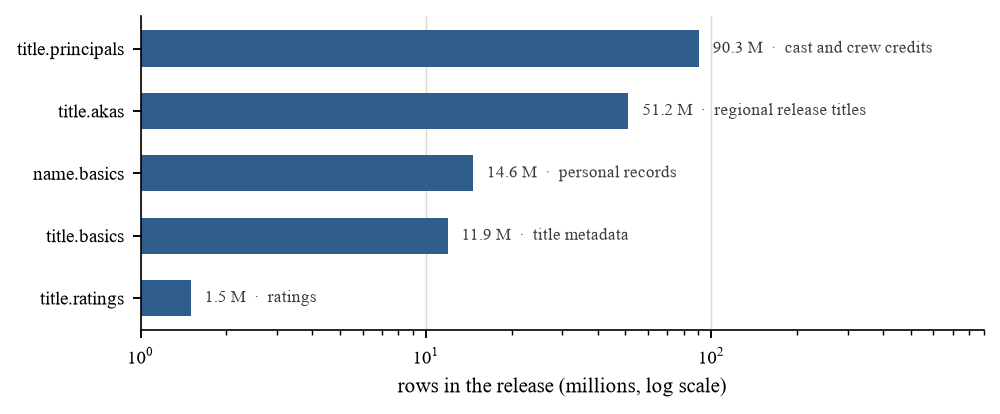
\includegraphics[width=\linewidth]{figures/fig02_dataflow.png}
\caption{Rows contributed by each source file; the principal-credits file alone accounts for 53\% of the scan.}
\end{figure}
